\documentclass[../main.tex]{main.tex}
\begin{document}
\section{Altermagnetism}
\subsection{Introduction and overview}
The reader might already be familiar with ferromagnets and all the regular magnetic models. Taking into account the spin and
wave vector of each particle in a site, one can derive some symmetries under transform operations. For example a
ferromagnet is symmetric under time-reversal and spin-rotation. In the example of the antiferromagnetism,
we have two sub-lattice with opposite spins. In such systems the spin compensate each other resulting in a null magnetization.
The system is symmetric under spin-flip and translation, and was theorized in 1948 by Louis Néel as the Néel antiferromagnets \cite{Neel1936}.
Allowing more complexity one could imagine multiple ions in a unit cell linked by symmetries such as rotation and screw operations. Half of the ions in the cell
own an opposite spin from the other half. The spectra compensate each other resulting in a zero net magnetization.
Moreover, these mediums keep the same electron spectra under such transformations, making them the same as Néel's antiferromagnets.
These material are labelled as zero $q$ antiferromagnets.
This section summarizes the historical work of \cite{Mazin2024}.\\

Altermagnets implement two or more sub-lattice which are not related between each other by translation or inversion.
The symmetry that actually links these sublattices is a rotation,
along with a spin-polarisation in the momentum space linked with a rotation as well \cite{Smejkal2022}.
In general, rotation doe not conserve the electrons spectra. We actually observe a band splitting of the spectra with respect to the spins.
There is an alternating sign in the spin-splitted momenta, as well as an alternating spin of the polarization in real space,
which leads to the name altermagnetism \cite{Smejkal2022_2}. This class of material was discovered in 2019 \cite{Hayami2019}.
\begin{figure}[H]
    \centering
    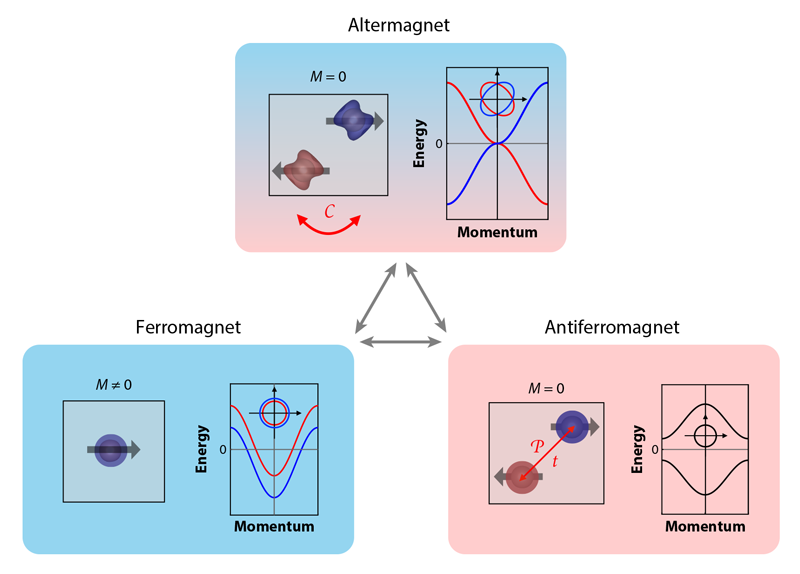
\includegraphics[width = 0.75\textwidth]{Ressources/AM.png}
    \caption{The altermagnet shares similar properties with the antiferromagnets like two sublattices of opposite spin, resulting in a zero net
    magnetization. Whereas the antiferromagnet's sublattices are liked by a translation $t$ and a space inversion $\mathcal{P}$, in the altermagnet one can link
    each sublattice with a rotation, here labelled as $\mathcal{C}$. We observe as well an alternating sign in the energy spectra of both altermagnet's sublattices. 
    The credits for the figure go to \cite{Smejkal2022} and \cite{Stonebraker}.}
\end{figure}


These properties put the altermagnet in between
the conventional dichotomy of ferromagnets and antiferromagnet. In fact the altermagnet compensate its magnetical moments taking advantage of the two
sublattices, like the antiferromagnet does. On the other hand, it shares similar properties with the ferromagnets, such as anomalous Hall effect,
spin current \cite{Naka2021_2}, magneto-electric effect \cite{Smejkal2022_3} and tunnelling magnetoresistance \cite{Smejkal2022_4} among other processes \cite{Smejkal2022_2}.\\

% Now that we have a better understanding of altermagnetism we can compare it with another class of material, where the sublattices
% aren't linked with the conventional crystal symmetries.
% As a consequence summing up the spin might not result in a trivial expression like the antiferromagnetic material. In fact the overall
% spin projection might almost be zero but not exactly. However, studying half metal and insulator leads to different result.
% Half metal can be seen as an insulator in one spin channel 
% but not both \cite{Mazin2024}. The Quin Luttinger's theorem, showed that such substance must have an integer number of Bohr spin
% magnetic moment. Therefore, structures with a small net magnetization see these quantities be floored to zero. \\

A few materials seem to exhibit these properties. 1D material will not work because of the lack of rotation possibilities. A diverse list of two and three-dimensional 
materials were listed by \cite{Smejkal2022}. We can cite semimetals with a Cr$_2$O monolayer \cite{Chen_2023}, a variety of insulators like 
perovskite oxide LaMnO$_3$ \cite{Yuan2021} CaCrO$_3$ \cite{Naka2021}, ferrite  Fe$_2$O$_3$ \cite{Smejkal2022_2}, or organic insulators $\kappa$-Cl \cite{Naka2019}.
We find as well the chalcogenide MnTe semiconductor \cite{Smejkal2022_2}.

On the sake of practical application, researchers have found (an exhaustive list is provided in \cite{Mazin2024}) that
domain like tunnelling magnetoresistance (TMR) are limited under the properties of the material. For instance the actual use 
of ferromagnets limits the frequency to the gigahertz range \cite{Mazin2024}.
This has to deal with the ferromagnetic resonance that connects 
the magnetization with electromagnetic waves. The altermagnets could be used in the terahertz range.
Mentioning that TMR is a key component of the magnetic random access memory (MRAM) \cite{OSullivan2004}\cite{Yadav2022}, the reader can easily estimate the performance
improvement such upgrade could deliver in a computer.\\
 
After this introduction on altermagnets, we intend to find a way to implement these into our system. In a more formal way, we can
distinguish two types of altermagnet.
In the first type, the altermagnet's lattice site have different distance to the neighbours depending on the linking axis and the 
spin of the particle in the site. This is illustrated in Fig. \ref{fig:altermagnet_lattice} $(\bm{a})$. On the other hand, we can consider a unit cell being unsymmetrical
in its ion position. We consider a square lattice were each unit cell has a non-magnetic ion and two magnetic ions with opposite spins.
Please consider the second schema $(\bm{b})$.\\

\begin{figure}[H]
    \centering
    \begin{tikzpicture}
        % Define the distance between the two graphs
        \pgfmathsetmacro{\distance}{7}; % Adjust this value to control distance

        % First graph (Altermagnet type 1)
        \begin{scope}
            \coordinate (o) at (0,0);
            \foreach \sign in {-1, 1}
            {
                \foreach \dir/\col/\title/\pos in {2/TamYellow/t+m/above, 0.75/TamLightGreen/t-m/left}
                {
                    \pgfmathparse{ifthenelse(\dir==2, \dir*\sign, 0)} % Calculate x-coordinate
                    \let\x=\pgfmathresult
                    \pgfmathparse{ifthenelse(\dir==2, 0, \dir*\sign)} % Calculate y-coordinate
                    \let\y=\pgfmathresult

                    % Use the computed coordinates in a let statement
                    \coordinate (a) at (\x,\y);               
                    \draw[-, color = \col, very thick] (o) --  (a) ;
                    \ifthenelse{\equal{\sign}{-1}}{\ifthenelse{\equal{\dir}{2}}{
                        \node[\pos, color = \col!70!black] at ($ (o)!0.5!(a) $) {\(\title\)};
                    }{
                        \node[\pos, color = \col] at ($ (o)!0.5!(a) $) {\(\title\)};
                    }}{}
                    \filldraw[color=black, fill=white, thick] (a) circle (0.1);
                }
            }
            \filldraw[color=black, fill=white, thick](0,0) circle (0.2);
            \node[anchor=center] at (o) {\(\scriptsize\uparrow\)};
            \pgfmathsetmacro{\shift}{3.5}
            \coordinate (o2) at (0 + \shift ,0);
            \foreach \sign in {-1, 1}
            {
            \foreach \dir/\col in {2/TamYellow, 0.75/TamLightGreen}
                {
                \pgfmathparse{ifthenelse(\dir==2, 0,\dir*\sign )} % Calculate x-coordinate
                \let\x=\pgfmathresult
                \pgfmathparse{ifthenelse(\dir==2, \dir*\sign ,0)} % Calculate y-coordinate
                \let\y=\pgfmathresult
                
                % Use the computed coordinates in a let statement
                \coordinate (b) at (\x + \shift ,\y);               
                \draw[color = \col , very thick] (o2) -- (b) ;
                \filldraw[color=black, fill = white , thick] (b) circle (0.1);
                    
                }
            }
            \filldraw[color=black, fill = white , thick](0 + \shift ,0) circle (0.2);
            \node[anchor=center] at (o2) {\(\scriptsize\downarrow\)};
        \end{scope}

        % Second graph (Altermagnet type 2)
        \begin{scope}[xshift=\distance cm] % Shift the second graph down
        \coordinate (o) at (0,0.5);
        \coordinate (a) at (1,0.5); % Added 0.5 to y-coordinate
        \coordinate (b) at (1,-0.5); % Added 0.5 to y-coordinate
        \pgfmathsetmacro{\size}{0.5}
        \coordinate (cell) at (-\size , \size + 0.5); % Added 0.5 to y-coordinate
        \filldraw[color=black, fill=white , thick] (o) circle (0.2);
        \node[anchor=center] at (o) {\(\scriptsize\uparrow\)};    
        \filldraw[color=black, fill=gray!30 , thick] (a) circle (0.1);
        \filldraw[color=black, fill=white , thick] (b) circle (0.2);
        \node[anchor=center] at (b) {\(\scriptsize\downarrow\)}; 

        \pgfmathsetmacro{\size}{0.3}           % Set the size for the offset
        \pgfmathsetmacro{\step}{1 + 2*\size} % Precompute the step size
        % Define the initial coordinate
        \coordinate (cell) at (-\size, \size + 0.5); % Added 0.5 to y-coordinate

        % Calculate each vertex position relative to (cell)
        \coordinate (p1) at ($(cell) + (\step, 0)$);
        \coordinate (p2) at ($(p1) + (0, -\step)$);
        \coordinate (p3) at ($(p2) + (-\step, 0)$);

        % Draw the dotted path using the calculated points
        \draw[-, dotted] (cell) -- (p1) -- (p2) -- (p3) -- cycle;

        \coordinate (lattice) at (2,-0.5);         % Adjusted y-coordinate
        \pgfmathsetmacro{\lattice}{0.5};         % Set the lattice size
        \pgfmathsetmacro{\numPoints}{3};         % Define the number of points in the lattice
    
        \foreach \x in { 0, 1,2} {               % Loop over x-coordinates
            \foreach \y in {-1,0, 1} {           % Loop over y-coordinates
                \coordinate (current) at ($(lattice) + (\x*\lattice, \y*\lattice + 0.5)$); % Added 0.5 to y-coordinate
                
                % Calculate fade component based on distance from (2,2)
                \pgfmathsetmacro{\scale}{100 - 10*sqrt((\x-2)^2 + (\y-2)^2)};
                
                % Ensure \scale is within valid color range
                \pgfmathsetmacro{\scaleClamped}{max(0, min(100, \scale))}; % Clamp between 0 and 100

                % Draw the filled circle with the calculated color
                \filldraw[fill=TamYellow!\scaleClamped!black] (current) circle (0.1); % Draw the circle
            } % End of y loop
        } % End of x loop
        \draw[dotted] ($(p1) + (0.15,0)$) -- ($(lattice) + (0,\lattice) + (0, 0.1)$);
        \draw[dotted] ($(p2) + (0.15,0)$)  -- ($(lattice) + (0,\lattice) - (0, 0.1)$);
    \end{scope}

    % Add labels (a) and (b)
    \node at (1.5, -2.5) {\(\bm{(a)}\)}; % Adjust position as needed
    \node at (\distance + 1.75, - 2.5) {\(\bm{(b)}\)}; % Adjust position as needed
    \coordinate (gizmo) at (-2,-2.5);
    \draw[->, thick] (gizmo) -- ++(0.75,0) node[anchor = west] {\(x\)};
    \draw[->, thick] (gizmo) -- ++(0,0.75) node[anchor = south] {\(y\)};
    \end{tikzpicture}

    \caption{Altermagnet of type 1 and 2.}
    \label{fig:altermagnet_lattice}
\end{figure}    

\subsection{Symmetries}
After giving an introduction on the geometric background of altermagnet we can now focus on the symmetries of the material. In this section
we are going to focus on two simple transformation. The inversion $P$ and the spin flip (time reversal) $T$ which are broadly discussed in the literature \cite{Smejkal2022}\cite{Smejkal2022_2}.
\begin{alignat*}{2}
    P : \bm{r} &\mapsto -\bm{r} ~~~~~~~~~~~~~~~~~~~~ &~~~\realnum^3 \rightarrow \realnum^3, \\
    T : t &\mapsto -t  ~\hat{=} ~\sigma \mapsto \overline{\sigma} &\realnum \rightarrow \realnum,
\end{alignat*}
with $\overline{\sigma}$ the opposite spin of $\sigma$.
We can first assume that the energy $\epsilon$ of the particle (or band structure) depends on the spin $\sigma$ and the wave vector $\bm{k}$. The equation $\bm{p} = \dd \bm{r}/\dd t$ and the de Broglie hypothesis 
$\bm{p} = \hbar\bm{k}$ \cite{Broglie1924} can lead to: 
\begin{align*}
    P \bigl(\epsilon(\bm{k}, \sigma)\bigr) &= \epsilon(-\bm{k}, \sigma)\\
    T \bigl(\epsilon(\bm{k}, \sigma)\bigr) &= \epsilon(-\bm{k}, \overline{\sigma})
\end{align*}
We observe the $PT$ operation $P\circ T$. If the system is $PT$ symmetric, one should get $\epsilon(\bm{k}, \sigma)= P\circ T\bigl(\epsilon(\bm{k}, \sigma)\bigr)$.
Assuming it's the case we can write
\[
    \epsilon(\bm{k}, \sigma)= P\circ T\bigl(\epsilon(\bm{k}, \sigma)\bigr) =  \epsilon(\bm{k}, \overline{\sigma})
\] 
and therefore the $PT$-symmetric systems are spin-degenerated. We have the same energy for a given momentum at two opposite spins.
 Reciprocally this means that the existence 
of $ \epsilon(\bm{k}, \sigma)$ is followed by an observation of $ \epsilon(\bm{k}, \overline{\sigma})$.\\

\paragraph{A few examples}$~$\\

To illustrate these symmetries we can consider a few examples.
We can imagine having a small lattice section for the sake of readability. First we choose a ferromagnetic lattice, where we apply the space inversion
in the middle, on the black cross. The arrows represent the spin and the overall sign of the wave vector $\bm{k}$ is given under each state. Moreover, 
we use the shading to keep track of the real space location of the site. This representation is in the real space.\\
\begin{figure}[H]
    \centering
        \begin{tikzpicture}
            \begin{scope}
            \coordinate (0) at (0,0);
            \pgfmathsetmacro{\lattice}{0.5};         % Set the lattice size
            \foreach \shift in {0,3.5,7}{
                
                \ifthenelse{\equal{\shift}{3.5}}
                {
                    \node[anchor = center] at ($(\shift + \lattice, -0.75)$) {\(-\bm{k}\)};
                }{
                    \node[anchor = center] at ($(\shift + \lattice, -0.75)$) {\(\bm{k}\)};
                }
                
            \foreach \x in {0,1,2} {               % Loop over x-coordinates
            \foreach \y in {0,1,2} {           % Loop over y-coordinates
                \coordinate (current) at ($ (\x*\lattice + \shift, \y*\lattice)$); % Added 0.5 to y-coordinate
                
                % Calculate fade component based on distance from (2,2)
                \pgfmathsetmacro{\scale}{(\x+\y)/4 * 100};                
                % Ensure \scale is within valid color range
                

                \ifthenelse{\equal{\shift}{3.5}}{\node[anchor = south] at ($(current)+ (0,-0.1)$) {\(\uparrow\)};}{
                    \ifthenelse{\equal{\shift}{7}}
                        {\node[anchor = south] at ($(current)+ (0,-0.1)$) {\(\uparrow\)};}
                        {\node[anchor = north] at ($(current)+ (0,0.1)$) {\(\downarrow\)};}
                }
                \ifthenelse{\equal{\shift}{7}}
                {
                    \pgfmathsetmacro{\scaleClamped}{100-max(0, min(100, \scale))}; % Clamp between 0 and 100
                    \filldraw[fill=TamYellow!\scaleClamped!TamLightGreen] (current) circle (0.1); % Draw the circle
                }{
                    \pgfmathsetmacro{\scaleClamped}{max(0, min(100, \scale))}; % Clamp between 0 and 100
                    \filldraw[fill=TamYellow!\scaleClamped!TamLightGreen] (current) circle (0.1); % Draw the circle
                }

            }
            }
            }
            \node[color=black, anchor=center, color=black] at (4, 0.5) {\(\times\)}; % Draw the circle
            \draw[->,semithick] (1.7,0.5) -- (2.7,0.5)  node[midway, above] {\(T\)};
            \draw[->,semithick] (5.2,0.5) -- (6.2,0.5)  node[midway, above] {\(P\)};
            \end{scope}

        \end{tikzpicture}

\end{figure}
The relevant variables for the symmetry in the spectrum are the spin projection and the momentum. We see, however, that the spin show a different spin orientation before and after the $PT$-operation.
Letting the spins point downwards again will require to use an additional operation. Therefore, the ferromagnet is not $PT$-symmetric, and we observe no spin degeneracy as the
equation shows it.\\

The antiferromagnet has a spin switch in every direction. Here, when choosing a point to apply our operations to, we see that 
neither a lattice point nor a point in the middle on two sites lead to a $PT$ symmetry. As we see the spins points in different directions.
\begin{figure}[H]
    \centering
    \begin{tikzpicture}
        \coordinate (0) at (0,0);
        \pgfmathsetmacro{\lattice}{0.75};         % Set the lattice size
        \foreach \shift in {0,2.75,5.5}{
            
            \ifthenelse{\equal{\shift}{2.75}}
            {
                \node[anchor = center] at ($(\shift + \lattice/2 , -0.75)$) {\(-\bm{k}\)};
            }{
                \node[anchor = center] at ($(\shift + \lattice/2, -0.75)$) {\(\bm{k}\)};
            }
            
        \foreach \x in {0,1} {               % Loop over x-coordinates
        \foreach \y in {0,1} {           % Loop over y-coordinates
            \coordinate (current) at ($ (\x*\lattice + \shift, \y*\lattice)$); % Added 0.5 to y-coordinate
            
            % Calculate fade component based on distance from (2,2)
            \pgfmathsetmacro{\scale}{(\x+\y)/2 * 100};
            
            % Ensure \scale is within valid color range
            \ifthenelse{\equal{\shift}{0}}{\pgfmathsetmacro{\mod}{mod(\x + \y,2)}}{\pgfmathsetmacro{\mod}{mod(\x + \y + 1,2)}}


            \ifthenelse{\equal{\mod}{1.0}}
            {\node[anchor = south] at ($(current)+ (0,-0.1)$) {\(\uparrow\)};}
            {\node[anchor = north] at ($(current)+ (0,0.1)$) {\(\downarrow\)};}

            \ifthenelse{\equal{\shift}{5.5}}
            {
                \pgfmathsetmacro{\scaleClamped}{100-max(0, min(100, \scale))}; % Clamp between 0 and 100
                \filldraw[fill=TamYellow!\scaleClamped!TamLightGreen] (current) circle (0.1); % Draw the circle
            }{
                \pgfmathsetmacro{\scaleClamped}{max(0, min(100, \scale))}; % Clamp between 0 and 100
                \filldraw[fill=TamYellow!\scaleClamped!TamLightGreen] (current) circle (0.1); % Draw the circle
            }

        }
        }
        }
        \node[color=black, anchor=center] at (3.15, 0.375) {\(\times\)}; % Draw the circle
        \draw[->,semithick] (1.25,0.25) -- (2.25,0.25)  node[midway, above] {\(T\)};
        \draw[->,semithick] (4,0.25) -- (5,0.25)  node[midway, above] {\(P\)};  
    \end{tikzpicture}
\end{figure}
However, if we apply the inversion in the in-between, we observe something different.\\
\begin{figure}[H]
    \centering
    \begin{tikzpicture}
        \coordinate (0) at (0,0);
        \pgfmathsetmacro{\lattice}{0.75};         % Set the lattice size
        \foreach \shift in {0,2.75,5.5}{
            
            \ifthenelse{\equal{\shift}{2.75}}
            {
                \node[anchor = center] at ($(\shift + \lattice/2 - 0.5, -1.5)$) {\(-\bm{k}\)};
            }{
                \node[anchor = center] at ($(\shift + \lattice/2 - 0.25, -1.5)$) {\(\bm{k}\)};
            }
            
        \foreach \x in {-0.5,0.5} {               % Loop over x-coordinates
        \foreach \y in {-1,0} {           % Loop over y-coordinates

        \ifthenelse{\equal{\shift}{5.5}}
            {
                \coordinate (current) at ($ (-\x*\lattice + \shift, -\y*\lattice)$); % Added 0.5 to y-coordinate
            }{
                \coordinate (current) at ($ (\x*\lattice + \shift, \y*\lattice)$); % Added 0.5 to y-coordinate
            }
            
            
            % Calculate fade component based on distance from (2,2)
            \pgfmathsetmacro{\scale}{abs((\x+\y)/2 * 100)};
            
            % Ensure \scale is within valid color range
            \ifthenelse{\equal{\shift}{0}}{\pgfmathsetmacro{\mod}{abs(mod(\x +0.5 + \y,2))}}{\pgfmathsetmacro{\mod}{abs(mod(\x +0.5+ \y + 1,2))}}
            %\node[anchor = south] at ($(current)+ (0,-0.1)$) {\mod};
            \ifthenelse{\equal{\mod}{0.0}}
            {\node[anchor = south] at ($(current)+ (0,-0.1)$) {\(\uparrow\)};}
            {\node[anchor = north] at ($(current)+ (0,0.1)$) {\(\downarrow\)};}

            \ifthenelse{\equal{\shift}{5.5}}
            {
                \pgfmathsetmacro{\scaleClamped}{100-max(0, min(100, \scale))}; % Clamp between 0 and 100
                \filldraw[fill=TamLightGreen!\scaleClamped!TamYellow] (current) circle (0.1); % Draw the circle
            }{
                \pgfmathsetmacro{\scaleClamped}{max(0, min(100, \scale))}; % Clamp between 0 and 100
                \filldraw[fill=TamYellow!\scaleClamped!TamLightGreen] (current) circle (0.1); % Draw the circle
            }

        }
        }
        }
        \node[color=black, anchor=center] at (2.75, 0) {\(\times\)}; % Draw the circle  
        \draw[->,semithick] (0.75,0) -- (1.75,0)  node[midway, above] {\(T\)};
        \draw[->,semithick] (3.5,0) -- (4.5,0)  node[midway, above] {\(P\)};
    \end{tikzpicture}
\end{figure}
Applying the $P$ transformation around this point makes the antiferromagnets having a $PT$ symmetry. We see that the lattice site have moved, but only the spin and
the wave vector take part to the band $\epsilon$. We therefore have a degeneracy in the energy spectrum. Finding at least one point where the $PT$ 
symmetry works makes the system $PT$ symmetric.\\

If we now take a look at an altermagnets pictured in Fig. \ref{fig:altermagnet_lattice}, we have two different models to test. In the first one $\bm{(a)}$,
the effect of the time reversal $T$ makes the hopping change $m\rightarrow -m$. Then we find no point
to invert the system around so that this first model does not have a $PT$ symmetry. For the second one $\bm{(b)}$,
we can first invert all spins, but afterwards, inverting the space does not bring back the system in the original configuration.
In fact, neither applying the $P$ after $T$ on the lattice point, nor on the space in-between, leads to the lattice we began with. In both cases, the 
degeneracy is lifted, we have dissimilar energies for the different spin-orientation. This is the reason for the band splitting we discussed in the introducing 
paragraph.\newpage

\paragraph{Brief mention of the spin-orbit coupling} $~$ \\

We refer to spin-orbit coupling (SOC) as the interaction between the spin of the electron and the orbital motion. 
When SOC is discarded we observe a rotation symmetry around the spins. A rotation $R$ can turn the spin back after the application of $T$
resulting in a $RT$ symmetry. $RT\bigl(\epsilon(\bm{k},\sigma)\bigr) = \epsilon(-\bm{k},\sigma)$ must equal $\epsilon(\bm{k},\sigma)$.

If we now consider a collinear magnet without SOC, we have a $RT$ but no $PT$ symmetry. Under such circumstances the spin-splitting must be symmetric under 
$\epsilon(-\bm{k},\sigma) = \epsilon(\bm{k},\sigma)$ which describes an even band structure. Such systems are called inversion symmetric altermagnets.\\

\subsection{Implementation of an altermagnet}
After introducing the basic properties of an altermagnet, we now aim to describe this system with the already introduced formalism.
We are going to consider the first model involving a spin-dependent hopping. The Hamiltonian is given by \cite{Ouassou2023} as:
\begin{equation*}
    H_{AM} = -\sum_{\langle i, j\rangle\sigma\sigma'} \left(\bm{m}_{ij} \cdot \bm{\sigma}\right)_{\sigma\sigma'} c_{i\sigma}^{\dagger} c_{j\sigma'} 
\end{equation*}
involving $\bm{\sigma}=(\sigma_1, \sigma_2,\sigma_3)^T$ the Pauli matrices. $\bm{m}_{ij}$ is the actual spin dependent hopping term. If the connection line 
between the two sites $i$ and $j$ lies on the $\bm{e}_x$ axis, we have $\bm{m}_{ij} = m(0,0,1)$ and $\bm{m}_{ji} = m(0,0,-1)$ along $\bm{e}_y$. $m$ is 
the desired hopping amplitude, and $\bm{m}_{ij}$ scales and masks the Pauli matrices. $\sigma_3$ puts $m$ on the diagonal, and takes care of the sign switch. 
Now having the normal metal t-hopping and this term leads to the $t\pm m$ we
described in Fig. \ref{fig:altermagnet_lattice} (\textbf{a}).\\

Now that we have a better understanding of the superconductivity and the altermagnets, we can move on to the next section where we will present a method to self consistently solve
the gap. This will be done by diagonalizing the Hamiltonian, and read the superconductivity from the eigenvalues and -vectors. To do so we need to discretize the
system by introducing the tight binding model.
\end{document}